\section{Scoping and symbol tables}
Crucial to the implementation of the \textit{tainting dependencies} methodology
described in section \ref{sect:trans:taintingDependencies} is the ability to
maintain a contextual environment with scoping and symbol tables. This section
details the implementation of this, and how it is used to achieve the
requirements of \textit{tainting dependencies}.

\subsection{Concepts}
The scoping system in the implementation is based on building a scope tree. The
previous scope, if any, is set as parent of the new scope, and the previous
scope maintains a list of child scopes -- this is referred to as
\textit{pushing a scope}. When exiting a scoped subexpression in the AST, the
previous scope is again set as the current scope. This is referred to as
\textit{popping a scope}. A reference to the root scope node is always
maintained. Considering the example XQuery query in figure
\ref{fig:impl:scope_tree_ex_code}, the scope tree in figure
\ref{fig:impl:scope_tree_ex} is generated. The scope itself contains \emph{one}
symbol table for the current scope.

\begin{figure}[!htp]
\begin{center}
\begin{Verbatim}
for $i in (1,2,3) return 
  for $a in (4,5,for $b in (6,7,8) return $b) 
    return ($i,$a)
\end{Verbatim}
  \caption{Scope tree example code}
  \label{fig:impl:scope_tree_ex_code}
\end{center}
\end{figure}

\begin{figure}[!htp]
\begin{center}
  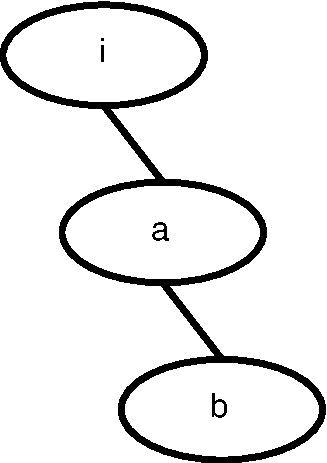
\includegraphics[width=0.2\textwidth]{diagrams/scope_tree_ex}
  \caption{Scope tree for source code in figure
  \ref{fig:impl:scope_tree_ex_code}} 
  \label{fig:impl:scope_tree_ex}
\end{center}
\end{figure}

Entries in the symbol table are represented through an instance of the
\texttt{SymTabEntry} class which maintains metadata about symbols (such as
symbol name, a flag indicating whether it's an iterator variable, and an
evaluated expression). The symbol table is realised as a subclass of the
\texttt{HashMap} class in the \texttt{java.util} package, and is constrained to
storing instances of \texttt{SymTabEntry}, with the symbol name as key.

\subsection{Semantics}
The scoping semantics are encapsulated in a singleton manner in the class
\texttt{Scope}, with static methods available for pushing and popping scopes,
and storing and retrieving symbols. The external (static) API as available to a
user of the scope system is shown in figure \ref{fig:impl:scope_uml}.

\begin{figure}[!htp]
\begin{center}
  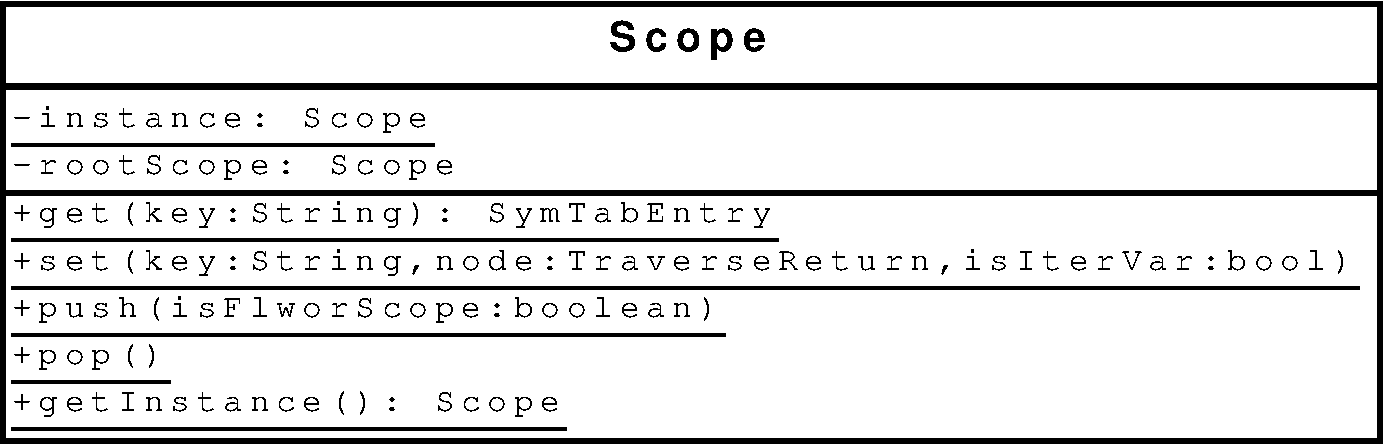
\includegraphics[width=0.7\textwidth]{diagrams/scope_uml}
  \caption{Scope API}
  \label{fig:impl:scope_uml}
\end{center}
\end{figure}

A new scope is \textit{pushed} whenever a for-clause is encountered while
parsing the abstract syntax tree, and the current scope is \textit{popped} while
evaluating a return clause -- both of which occur within a FLWOR expression.

The scoping system also tracks iteration variables. That is, for any scope,
there is \textit{one and only one} iteration variable, except in the top scope
where there is no iteration variable. The concept of an iteration variable is
explained in definition \ref{def:iterVarDep}. Tracking these
variables are necessary to implement the \textit{tainting dependencies}
methodology (explained later in section \ref{sect:impl:tainting_deps} on page
\pageref{sect:impl:tainting_deps}).